
\chapter{High Valence Vertices}\label{ch:high_valence}

High valence (HV) vertices are a mesh feature which cause significant degradation in
DAGMC ray tracing performance. The valence of a vertex in a mesh is defined as
the number of edges connected to that vertex. \textit{High} valence vertices are
defined as vertices connected to an unusually large number of edges. This
region, known as a HV region, will typically take on a fan-like shape
as seen in Figure \ref{fig:hv_examples}.  The geometric origins of HV
regions are typically a planar surface intersected with some form of curved
boundary condition. 

\begin{figure}[H]
  \centering
  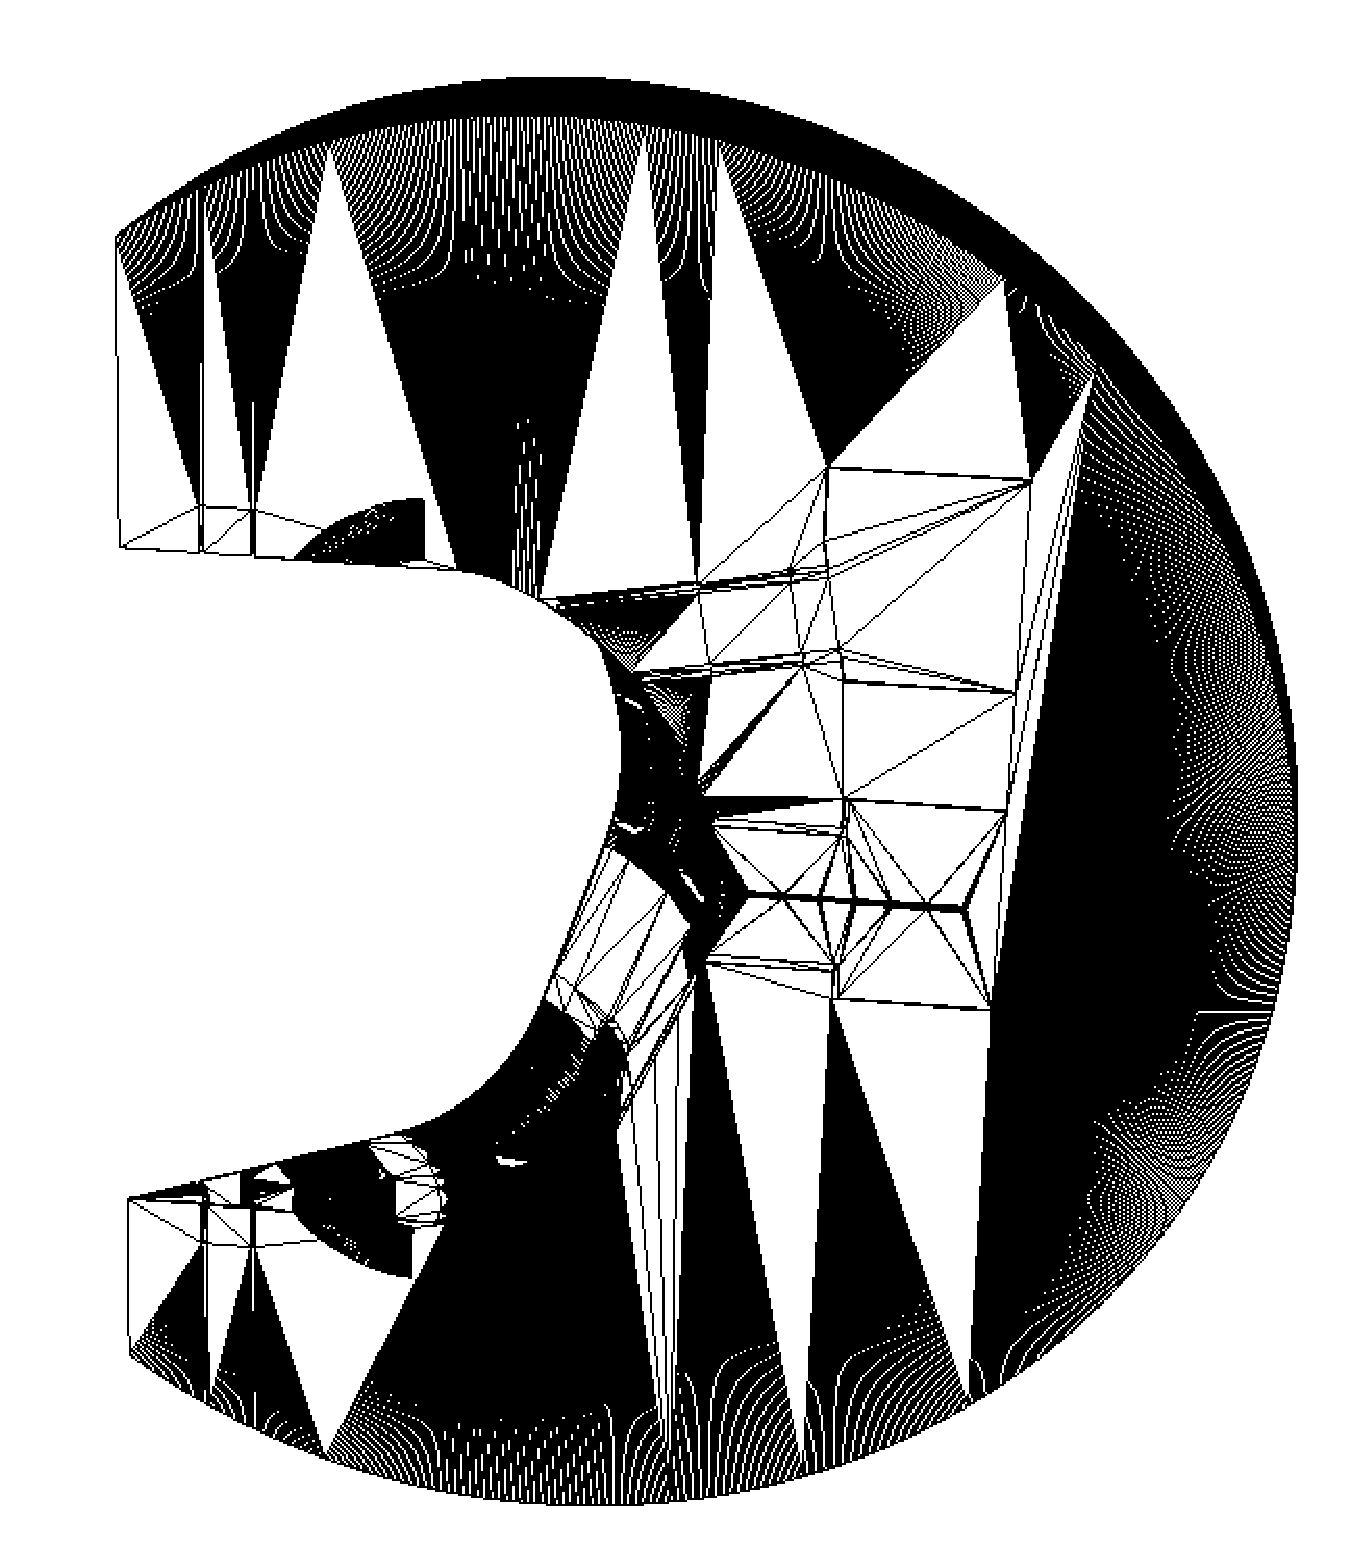
\includegraphics[scale=0.2]{iter_sideon.eps}
  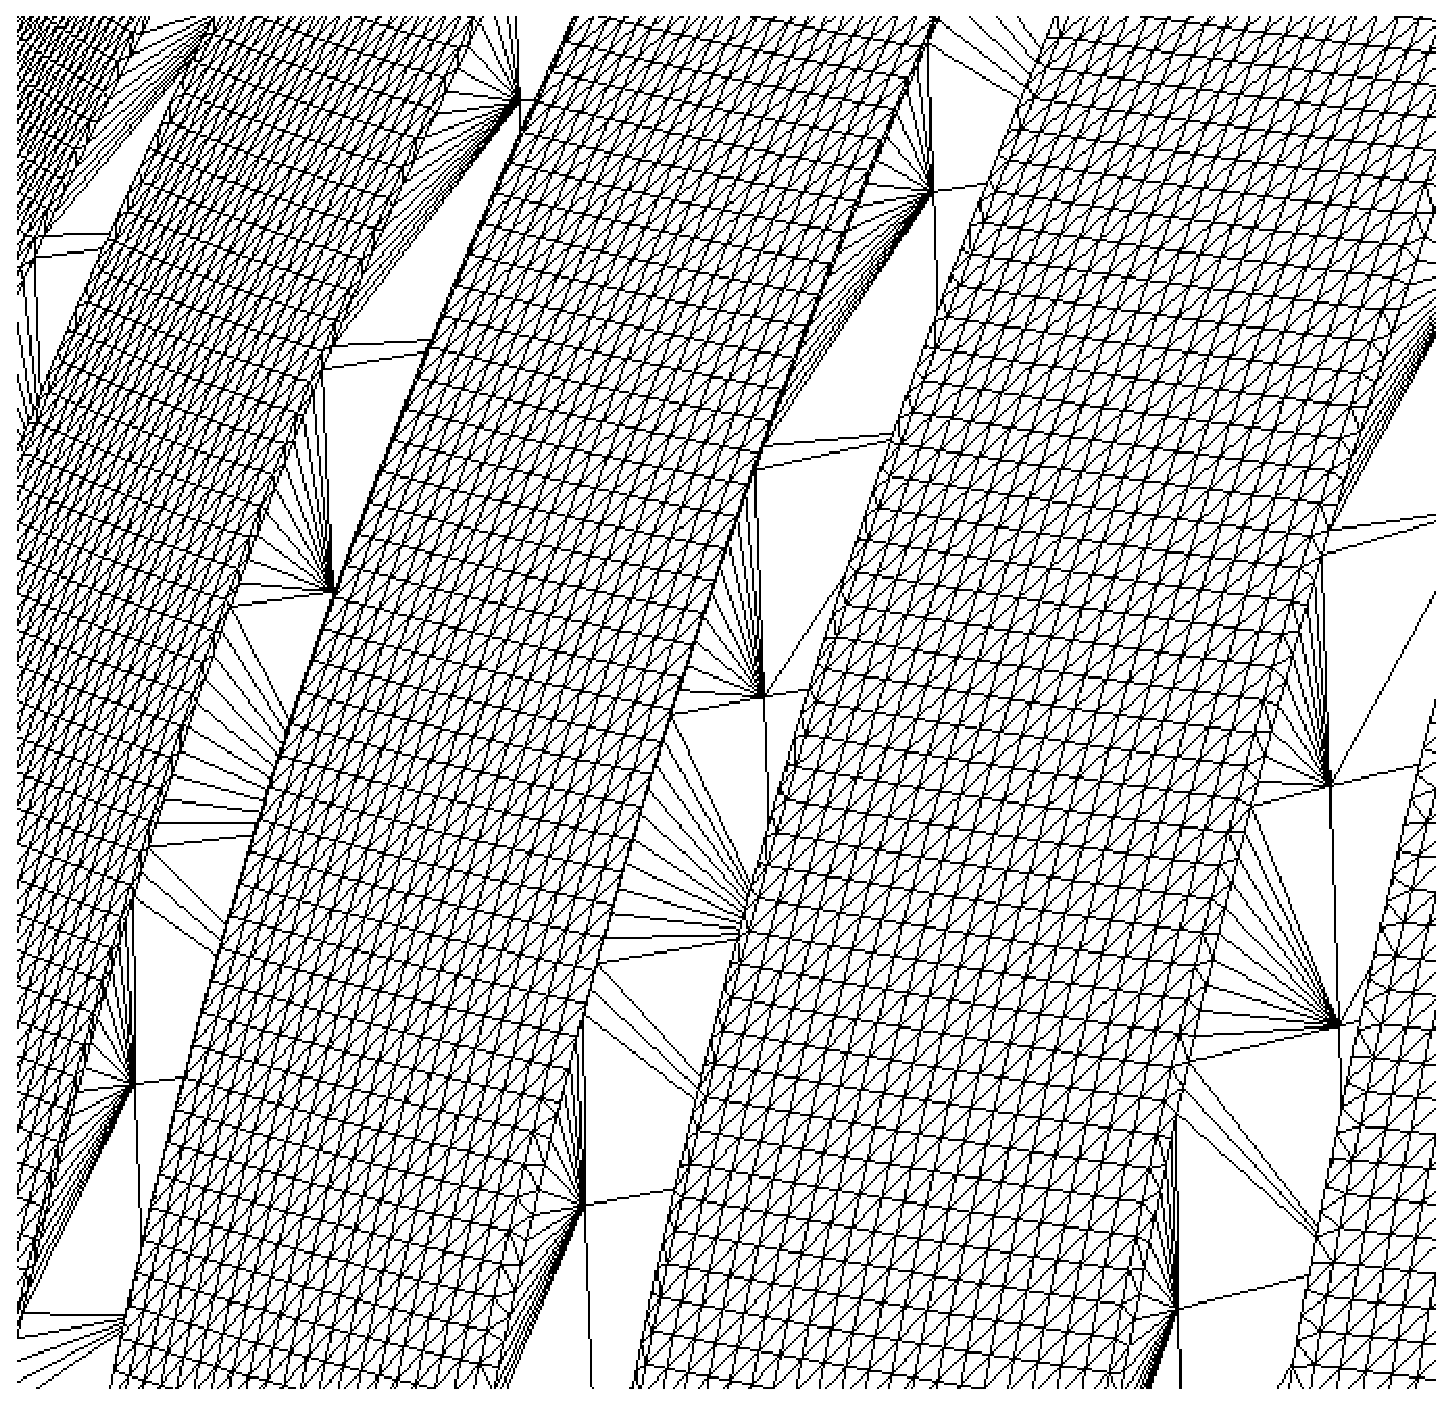
\includegraphics[scale=0.2]{ds_hv.eps}
  \caption[Examples of HV vertices in production models.]{Examples of HV
    vertices in production models.}
  \label{fig:hv_examples}
\end{figure}

These regions are commonly generated in the faceting algorithms used to produce
DAGMC meshes. This faceting scheme (which comes from ACIS libraries underlying
the CUBIT/Trelis geometry engine) is designed to produce the smallest number of
triangles possible to represent the model within the representation tolerance
specified in DAGMC's surface mesh generation preprocessing. This restriction is
favorable to the rasterization process commonly used to display models
interactively in CAD GUIs. Fewer triangles are better for the purpose
particle tracking in DAGMC as well as long as the geometry is accurately
represented. Even the ideal ray tracing acceleration structure queries for a
given triangle mesh scale as $O(log(N))$, and the size of models being analyzed
using the toolkit provides motivation to keep memory footprints as low as
possible. However, even with fewer triangles undesirable configurations can
impede performance as is shown by a set of tests conducted on models generated
by this faceting scheme.

\section{Previous Work}

A study conducted by Steve Jackson in 2010 on the performance of the MOAB OBB
tree revealed a steep degradation in performance with a decreasing faceting
tolerance or an increasing number of triangles \cite{Tautges_2009}. Using a
DAGMC-based ray fire test program, the performance of DAGMC's ray fire ability
was evaluated for four models. These models include a simple sphere, a notched
or slotted sphere, and an outer volume of an ITER model, shown in Figure
\ref{fig:sj_hv_test_models}.

\begin{figure}[H]
  \centering
    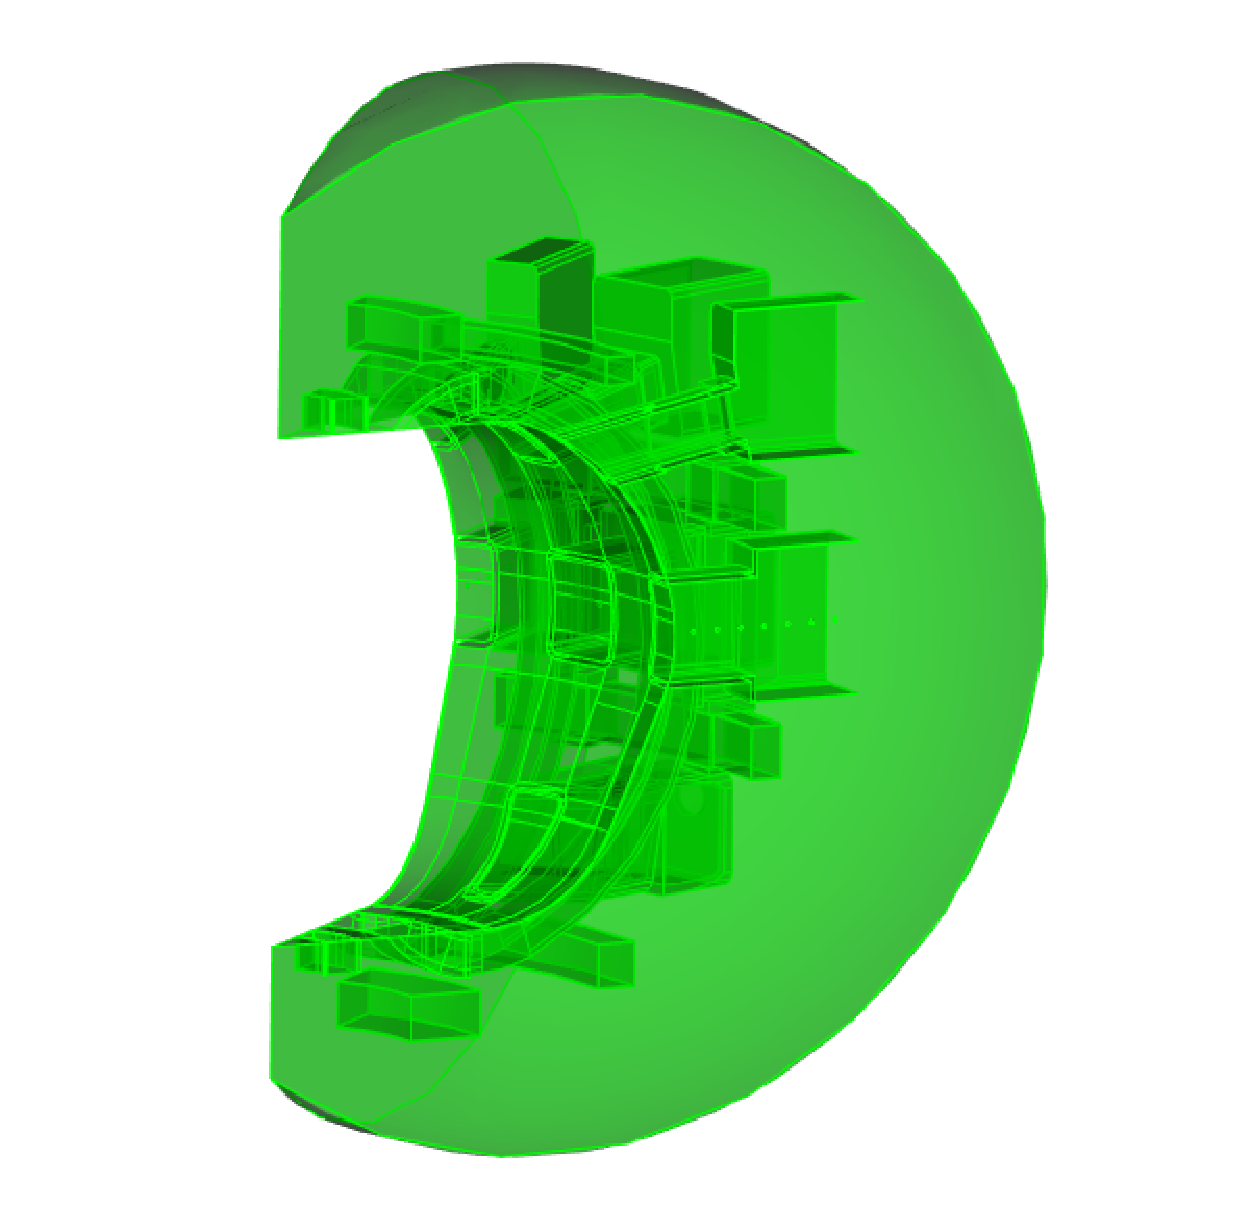
\includegraphics[scale=0.32]{iter_rf_vol.eps}
    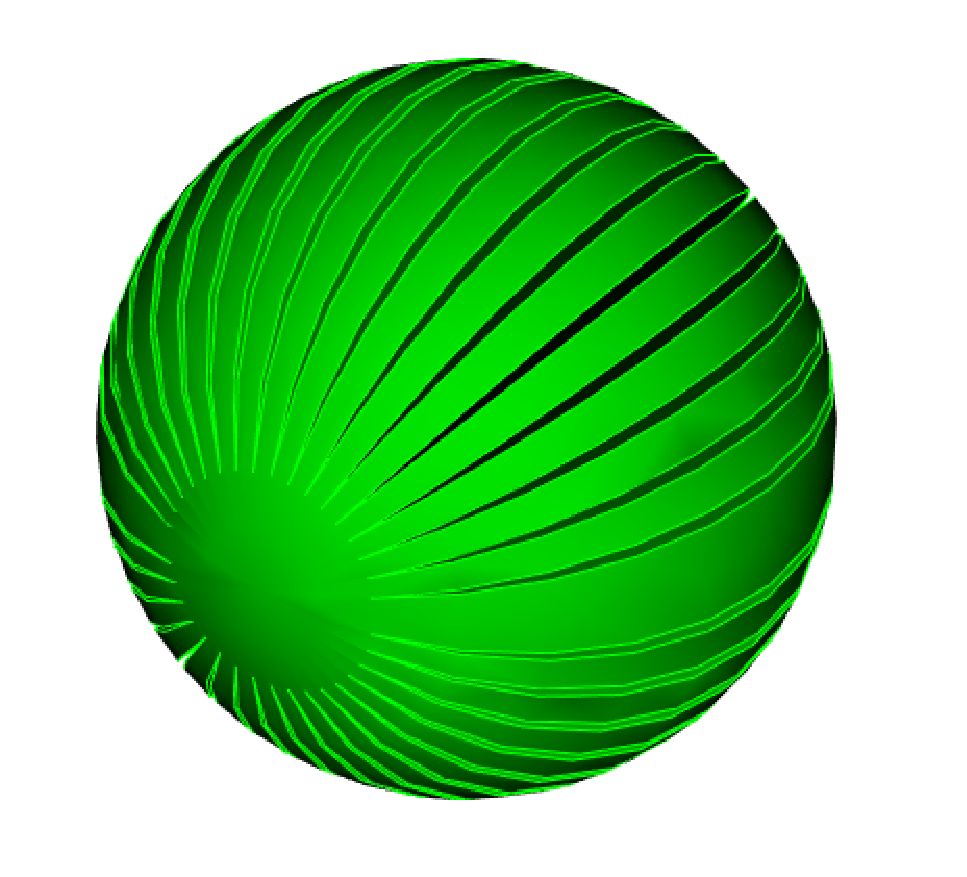
\includegraphics[scale=0.42]{ds.eps}
  \caption[CAD models used in ray fire timing.]{Images of the slotted sphere and
    ITER volume used to perform DAGMC ray fire performance tests with increasing
    number of triangles or, equivalently, decreasing faceting tolerance.}
  \label{fig:sj_hv_test_models}
\end{figure} 

In each of these tests, the models are tessellated with an increasingly smaller
faceting tolerance with the faceting tolerance being defined as the maximum
distance between the faceted curve or surface and the geometric curve or surface
it resolves. By this definition, the number of triangles needed to represent a
model scales inversely with the value of the faceting tolerance. An increase in
the number of triangles leads to a more complex nature of the surface mesh in
terms of BVH construction and traversal.

The first three models are identical to the ones used to measure ray fire times
in Chapter \ref{ch:simd_bvh}. Finally, the faceting of a volume from an ITER
model is used as a production demonstration of the effect of HV
regions on DAGMC performance (see Figure \ref{fig:hv_examples}).

\begin{figure}[H]
  \centering
  \begin{center}
    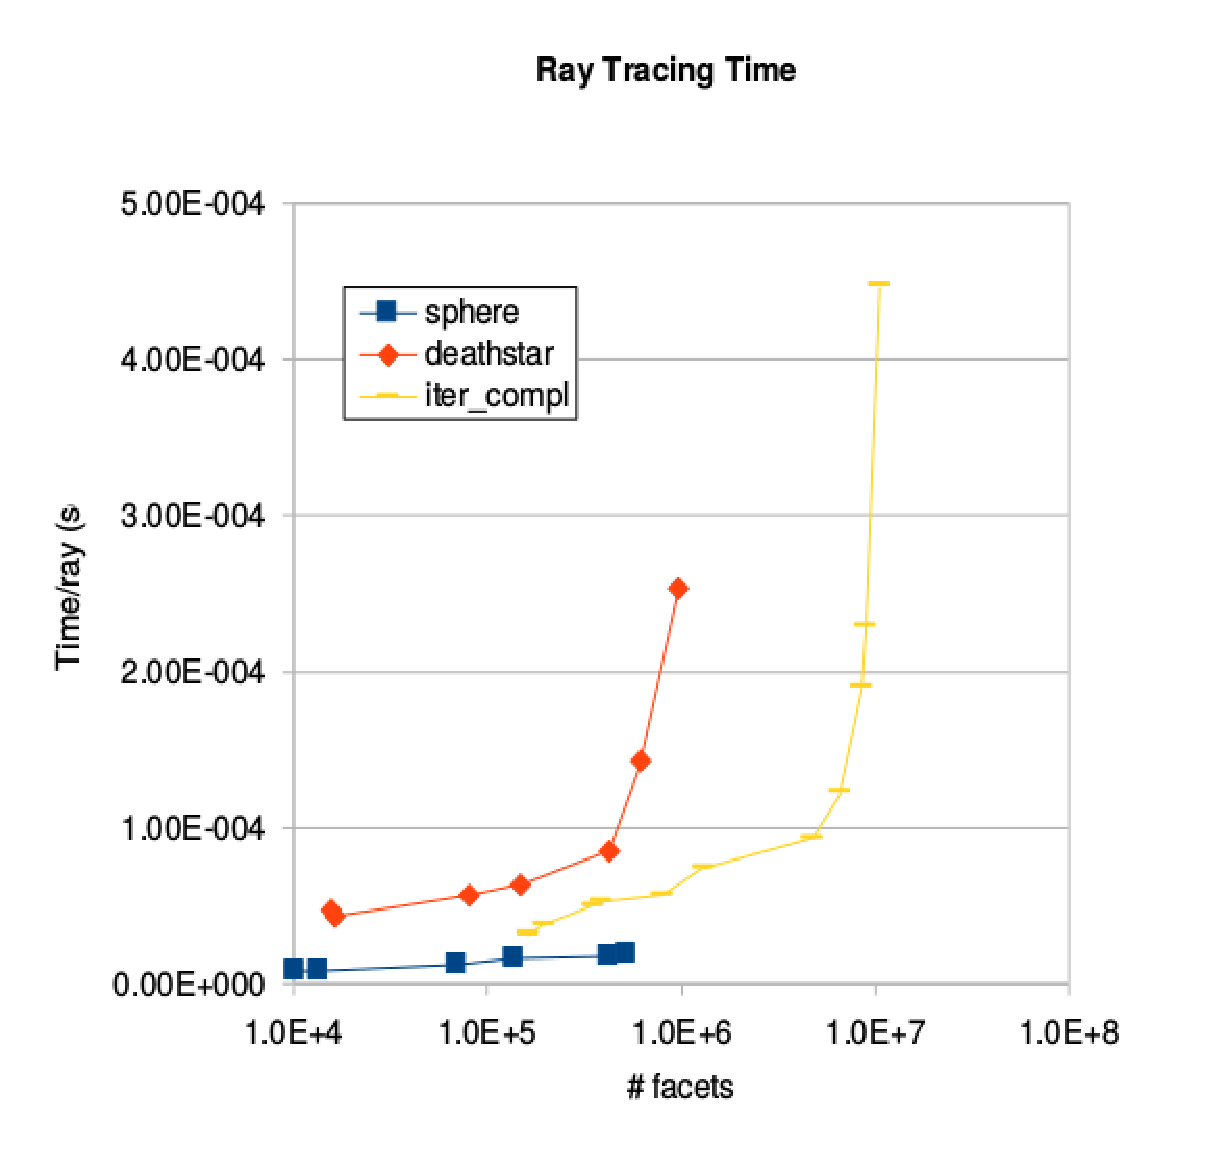
\includegraphics[scale=0.5]{sj_2010_orig.eps} \\
    \caption[Previous results of ray fire timings from 2010.]{Results of MOAB
      ray tracing performance tests with decreasing faceting tolerance performed
      by Steve Jackson in June of 2010. Data points represent average time spent
      in firing a ray for random rays originating at the center of each
      model\cite{Tautges_2009}. The ``deathstar'' model is the same as the
      slotted sphere model used in tests performed by the author.}
    \label{fig:sj_hv_test_results}
  \end{center}
\end{figure}

While the sphere model scales well with a decreasing faceting tolerance, the
ITER volume and slotted sphere both have a pronounced increase in average ray
fire time with decreasing faceting tolerance. Knowing that both of the latter
models contain HV regions, it was postulated at the time that these
regions had a significant effect on the scaling.

\begin{sidewaysfigure}
  \centering
  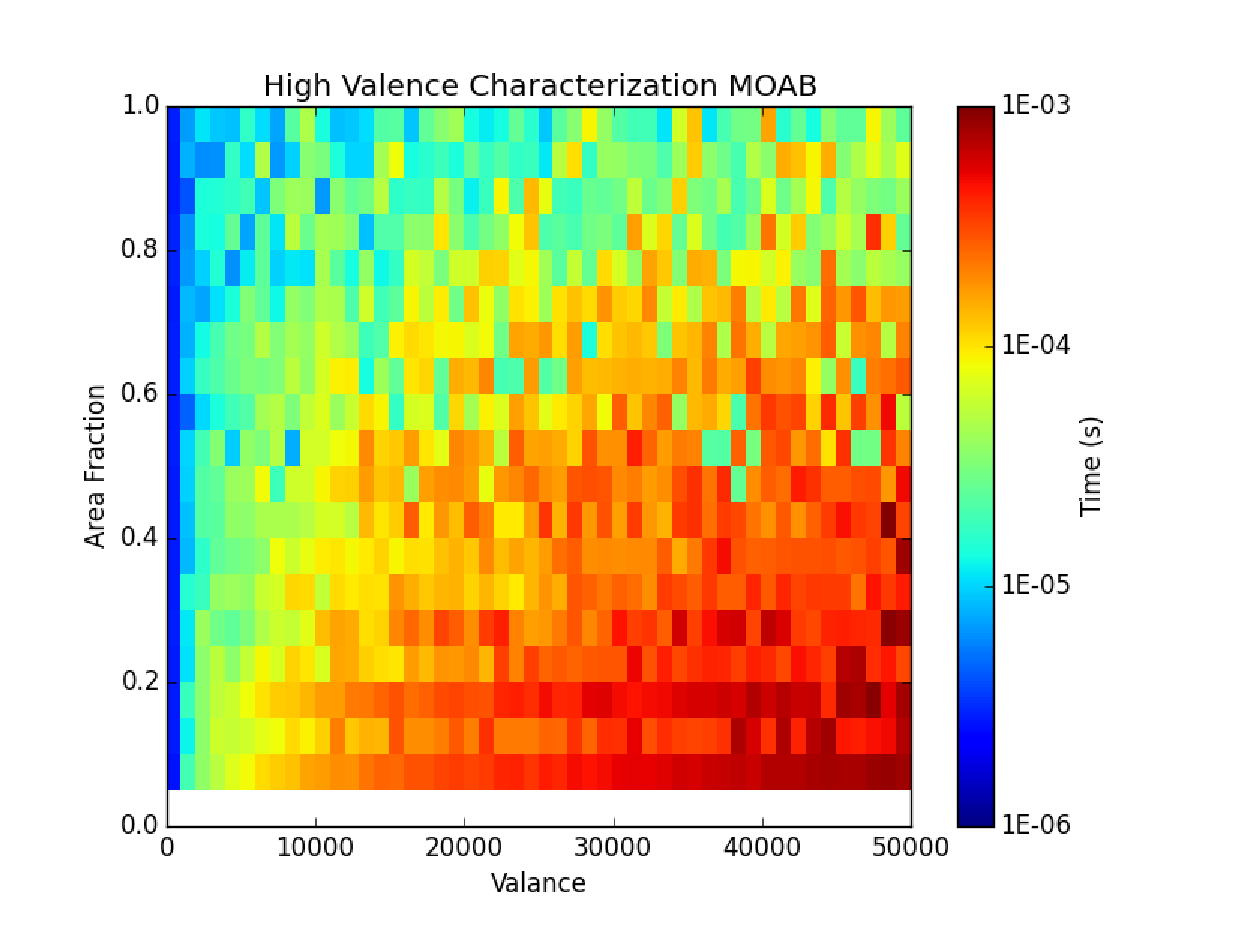
\includegraphics[scale=0.45]{hv_study_MOAB.eps}
  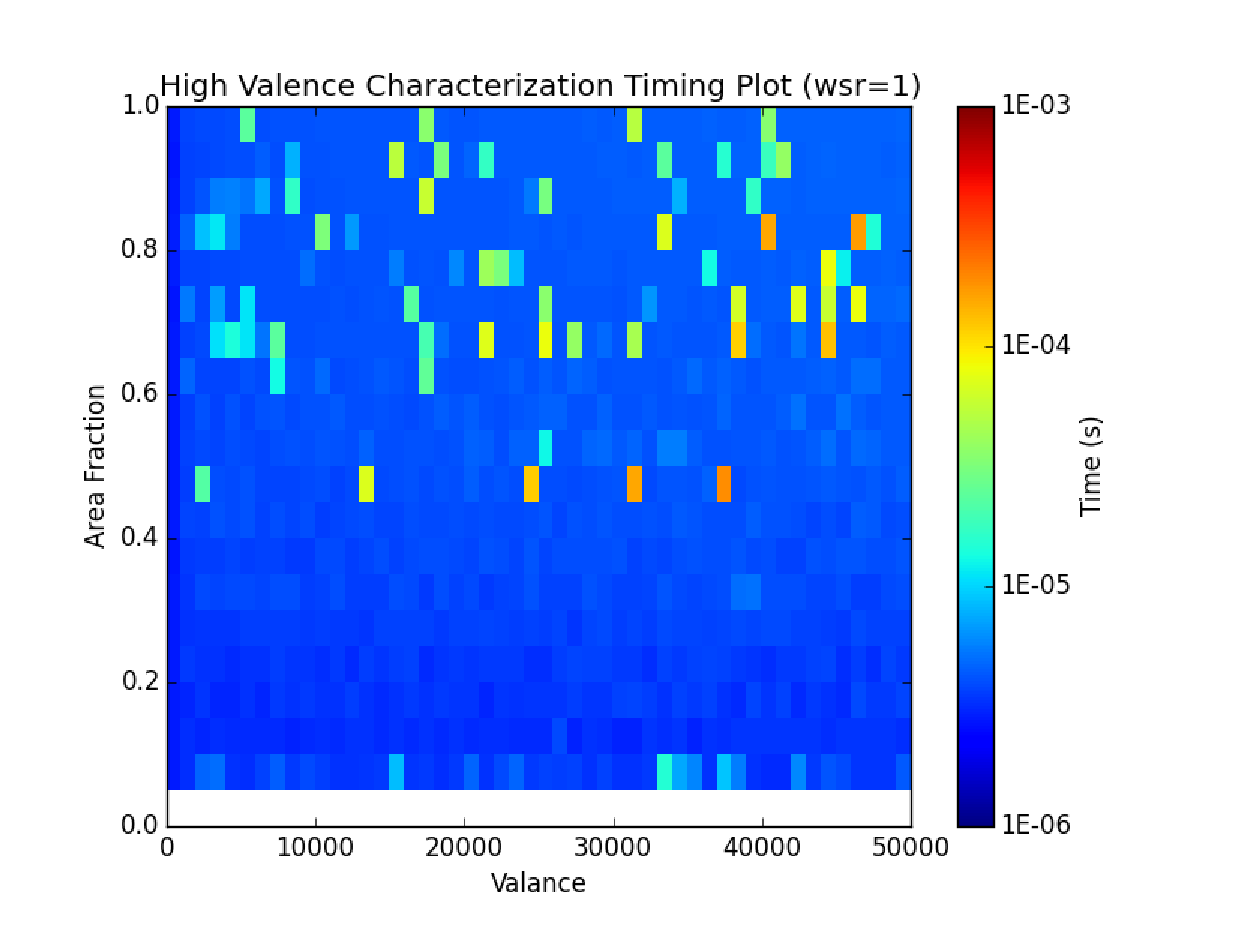
\includegraphics[scale=0.45]{hv_study_MOAB_wsr1.eps}
  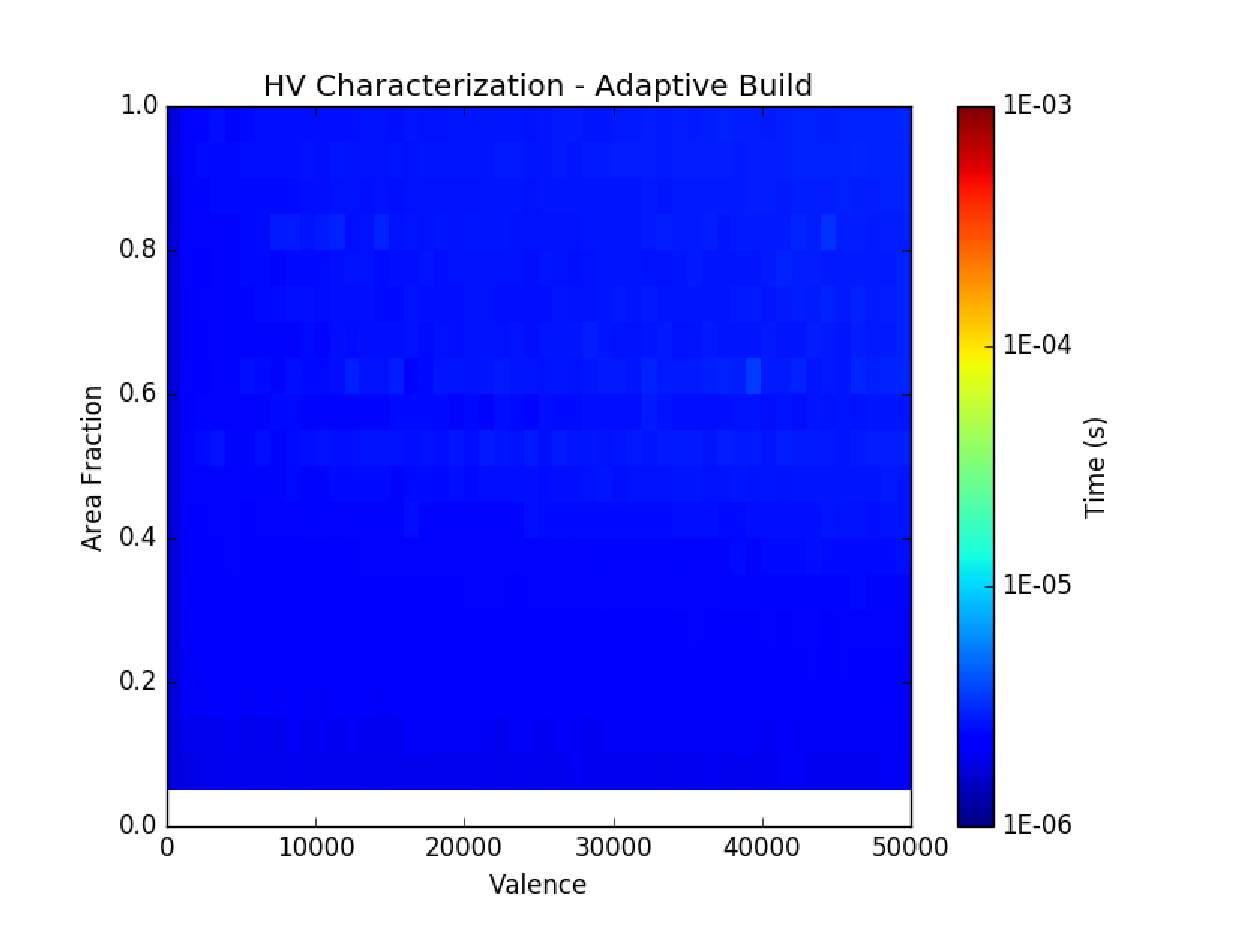
\includegraphics[scale=0.45]{hv_study_moab_adaptive.eps}
  \caption[High valence study results for various BVH implementations.]{HV characterization study
    results for all MOAB OBB tree implementations. Top Left: Unmodified MOAB
    results. Top Right: Manual modification of MOAB OBB tree's build
    settings. Bottom: Results with adaptive construction for HV regions.}
  \label{fig:moab_hv_studies}
\end{sidewaysfigure}

\section{High Valence Characterization Test Framework}

In order to isolate a HV region, a test model was manually generated in MOAB
with an artificial HV region (shown in Figure \ref{fig:hv_cube_design}). This
mesh is a modified cube mesh centered on the origin in which one of the
two-triangle surfaces has been replaced by a more complicated planar surface of
triangles including an interior HV region within the face. The HV region was
generated by inserting vertices along the diagonal of the interior box and
connecting them to the opposing corners of the box. This mesh is generated using
two input parameters: the valence of the corner vertices in the interior region
and the relative size of the interior region. A parametric study was then
performed by varying these two parameters in order to characterize the
performance impediment and determine its root cause.

\begin{figure}[H]
  \centering
    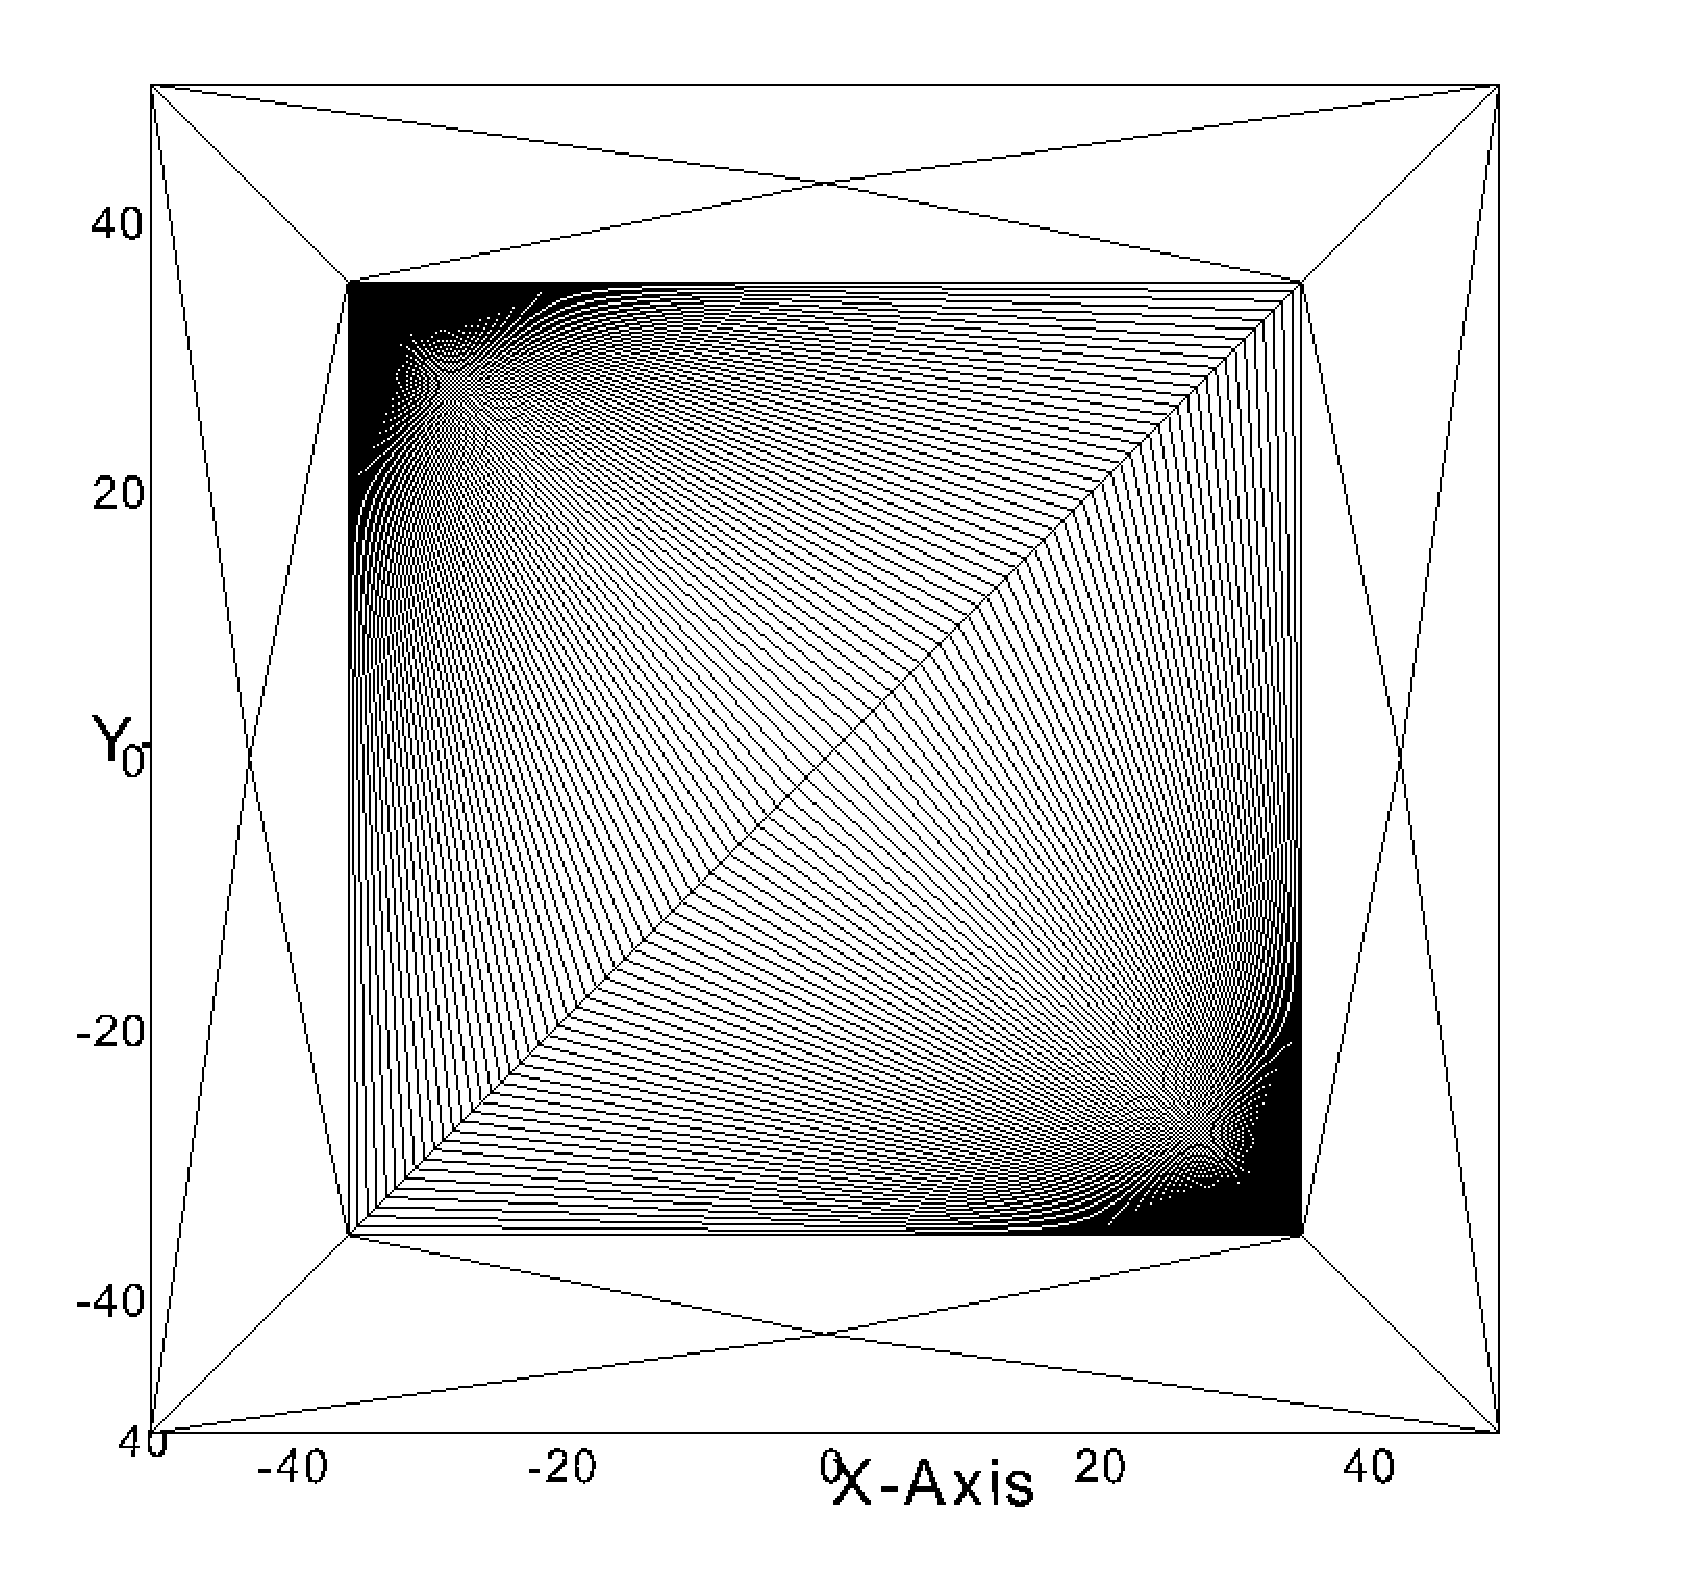
\includegraphics[scale=0.33]{hv_study_design.eps}
    \caption[High valence vertex test model.]{Side-on view of the modified cube
      mesh used to study the HV vertex problem.}
    \label{fig:hv_cube_design}
\end{figure}

DAGMC's ray fire test program was used to construct MOAB's BVH and perform ray
queries on this model. This program was used to fire rays with random
direction from the origin of the HV test model while biasing the ray directions
such that they are always incident upon the modified surface containing the HV
region. A parameter sweep was performed by varying the percentage of the surface
covered by the HV region as well as the valence of the region. Each test shown
in this section varies the valence of the corner vertices from 2 to 50,000 and
the relative area of the HV region from 0 to 1. Results of this study provided
insights into performance pathologies for various BVH implementations.

\section{MOAB's BVH}\label{sec:hv_study_MOAB}

From what is known about the construction of MOAB's OBB-BVH, it was expected
that the average ray fire time would be most strongly correlated to the relative
area of the HV region, but would also increase with increasing valence of the
corner vertices. The initial results of this study, shown in Figure
\ref{fig:moab_hv_studies}, meet only one of the expectations however. The ray
fire times become far worse with increase in valence, but for a constant
valence, the smaller relative area models show a longer average ray fire time
than the models with larger relative areas. This suggests that the presence of a
HV region in a surface is detrimental to performance regardless of the
likelihood that a ray intersects with a triangle in that region, which is
counter intuitive. In order to investigate this matter further, a visualization
tool for MOAB's BVH was developed to improve the author's intuition about this
mesh pathology.

\subsection{Visualization and Diagnosis}\label{subsec:hv_vis}

Using the same visitor pattern employed to traverse rays through the hierarchy,
each OBB in the HV model tree was converted into a hexahedral element and saved
in a VTK mesh format. Each hexahedron representing an OBB was tagged
with its depth in the tree as well as the triangle entities it contains, if it
is a leaf node. These mesh files can then be used to visualize the hierarchy
level-by-level and can be superimposed on the geometric mesh. An example of this
OBB visualization for the HV characterization model is shown in Figure
\ref{fig:bad_hv_box}.

\begin{figure}[H]
  \centering
    \includegraphics[scale=0.3]{{obbs_wsr_0.95}.eps}
    \caption[Oriented leaf bounding boxes in a high valence region.]{View of an
      OBB containing many HV region triangles as well as other
      surface triangles. Blue box and triangles: leaf node bounding box and
      associated triangles. Several thousand triangles are represented in the
      solid blue region shown here. Red boxes: Other representative OBBs at the
      same depth in that tree.}
    \label{fig:bad_hv_box}
\end{figure}

Because there are more entities to partition in the HV region, it is expected
the deepest levels of the BVH will contain only OBB's bounding triangles in that
region. It was expected that leaf nodes of the BVH might contain many triangles
of the HV region, causing performance degradation of ray traversal in that many
triangles must be checked for intersection. These types of poorly formed leaf
nodes shift the complexity of the BVH traversal back toward a linear search -
which is sub-optimal. This feature of MOAB's OBB tree were observed, but
visualization of the BVH provided the ability to observe another characteristic
as well. Many leaf nodes containing large numbers of triangles in the HV region
also contained one or two large triangles outside of that region. The inclusion
of these large triangles significantly increases the probability that a
hierarchy traversal will visit that leaf node and thus all of the triangles
contained by that leaf node. This artificial increase in the HV regions
cross-section greatly exacerbates the already poorly created nodes in the tree.

Due to the nature of the entity ratio heuristic used to divide nodes in the
tree, as the HV region becomes smaller more triangle centroids are
shifted onto one side of the median splitting planes used to divide the nodes
which contain portions of that region. If enough triangle centroids are on this
side of the plane, then the cost of the entity ratio evaluation will exceed the
preset upper limit of the cost (0.95 in MOAB) and the construction process will
declare that node a leaf node. The settings governing this split process can be
altered in MOAB, and changing the worst split ratio to 1.0 significantly
improves the average ray fire time in the HV characterization study,
as seen in Figure \ref{fig:moab_hv_studies}.

As expected, the use of this setting largely removes the degradation in performance
caused by the HV region by forcing the continued splitting of entities
in the tree where large leaf nodes would have been created before. This
demonstrates that altering this setting works well for this mesh feature, but it
would be detrimental to the memory footprint of the overall hierarchy in the
general case, causing portions of the OBB tree to be deeper than necessary. 


\subsection{Adaptive BVH Construction}\label{subsec:adaptive_construction}

One of the benefits to having a BVH tool which is part of a mesh database like
MOAB is the ability to query for more information about the mesh when
constructing hierarchies like the BVH. This information has been used to detect
HV regions in the mesh and adapt BVH construction to improve the
hierarchy quality in these areas.

\subsubsection{High Valence Detection}\label{subsubsec:hv_detection}

A simple algorithm is used to determine whether or not the entities inside a
leaf node are part of a HV region. Any vertex connected to more than a
user-defined proportion, $\alpha$, of the entities in a given leaf node will be
considered a HV region, indicating that an alternate build method or build
settings should be applied.

\begin{lstlisting}[language=Python,basicstyle=\tiny,caption={Algorithm for detecting HV regions.},label={alg:hv_detect},captionpos=b]
  def detect_hv_region(triangles, alpha):
      assert(a <= 1.0 and a > 0.0)
      connectivity = get_connectivity(triangles)

      for vertex in connectivity:
          # get all entities of dim 2 adjacent to the vertex
          adj_entities = get_adjacencies(vert, to_triangles)

          # determine the number of non-adjacent entities
          overlap = triangles - adj_entities

          if size(overlap)/size(triangles) < 1.0 - alpha:
              return true
      return false
\end{lstlisting}

\subsubsection{Implementation}\label{subsec:adaptive_construction_implementation}

First, MOAB's BVH constructor was modified to tag poorly
formed leaf nodes in the tree. This option will apply a tag to any leaf nodes
which contain more entities then specified in the settings for the tree. These
nodes are then revisited for further refinement later in the build process.

For handling of these poorly formed leaf nodes, a new class was created in MOAB
named the \textit{BVHRefiner}. This class visits each leaf node tagged by the
build process to determine if further refinement is appropriate based on the
available set of mesh features it is capable of adapting to. For each mesh feature
added to the BVH Refine class, a detection method and build method is
required. This class applies these detection methods and altered build methods
to resolve these leaf nodes into improved regions of the tree. The intent of
this design was to support the detection and adaptation to other pathological mesh
features in the future.

In the HV case, the refiner class was instructed to search for any vertex
connected to more than 80\% of the entities in that particular leaf node. If
this condition is met, the leaf node is declared part of a HV region and an
altered build method is applied. For the HV case, this build method has been
established by the characterization tests as the standard build algorithm with
the worst case splitting ratio set to the maximum value of 1.0.

\subsubsection{Application to the HV test model}

This adaptive build method was applied to the HV test model as before. The
results of this test can be seen in Figure \ref{fig:moab_hv_studies}. Using the
adaptive method, the average ray fire time is consistent across both valence and
relative area of the HV region and shows none of the stochastic behavior seen
when manually altering the tree's global build settings.

\subsubsection{Application to Production Models}

This method was applied to several DAGMC production models in order to determine
its effect on simulation run times during transport.

\begin{table}[H]
  \centering
  \begin{tabular}{c c c c c c}
    \toprule
    \textbf{\thead{Model}} & \textbf{\thead{HV \\ regions}} & \textbf{\thead{Run Time \\ reduction}} & \textbf{\thead{Build time \\ increase}} & \textbf{\thead{HV Leaf Visit \\ Relative Frequency}} \\
    \hline
    FNG            & 514                 & 24.2\%                      & 18.5\% & 3.83 \% \\
    ATR            & 755                 & < 3\%                       & 22.9\% & 0.07 \% \\
    UWNR           & 496                 & < 2\%                       & < 5\%  & 3.87 \% \\
    ITER           & 3522                & 29.4\%                      & 5.2\%  & 7.34 \% \\
    \bottomrule
  \end{tabular}
  \caption[Performance results for high valence region refinement in production models.]{Results of
    run time reduction in several DAGMC production models when applying the BVH
    refinement.}
  \label{tab:bvhrefine_production_results}
\end{table}    

As seen in Table \ref{tab:bvhrefine_production_results}, the ATR and UWNR
problem run time is decreased only marginally, but in the ITER and FNG models
the run time is reduced by $\approx\frac{1}{4}$. Given the outcome of this study
it might seem that the high valence regions are visited more often in the ITER
and FNG models, but information gathered during simulation using MOAB's mesh
tagging interface suggest otherwise. A sweep of the high valence parameter,
$\alpha$, for these models is shown in Figure \ref{fig:hv_parameter_study_moab}
which reflects the performance impact shown in Table
\ref{tab:bvhrefine_production_results}. It also describes the relationship
between the simulation run time and the high valence parameter value in the ITER
and FNG models. Even for a relatively high $\alpha$ parameter of 0.9, a
significant reduction in the run time is seen in these models. As the value
decreases, the run time is futher reduced to nearly 30\% of the maximum run time
in the study. The large change at a high value of $\alpha$ indicates that even
coarse detection of high valence regions has a measurable impact on performance.

\begin{figure}[H]
  \centering
  \includesvg{../images/hv_parameter_study_moab}{width=1.0\textwidth}
  \caption[High valence detection parameter study.]{Variation in run time for
    different HV detection parameters on a representative set of DAGMC models
    using the adaptive build method in MOAB.}
  \label{fig:hv_parameter_study_moab}
\end{figure}


\begin{sidewaysfigure}
  \centering
  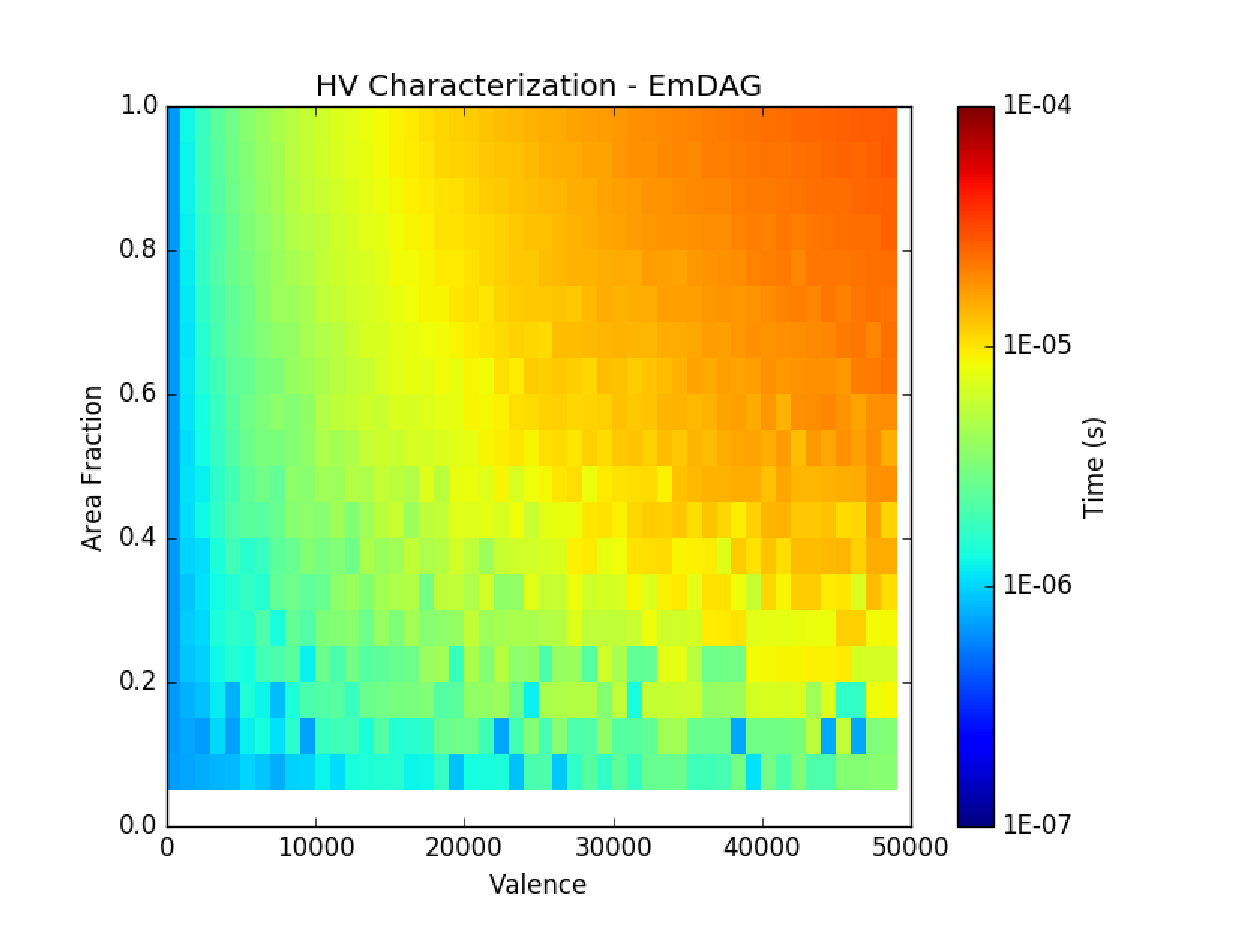
\includegraphics[scale=0.45]{hv_study_emdag.eps}
  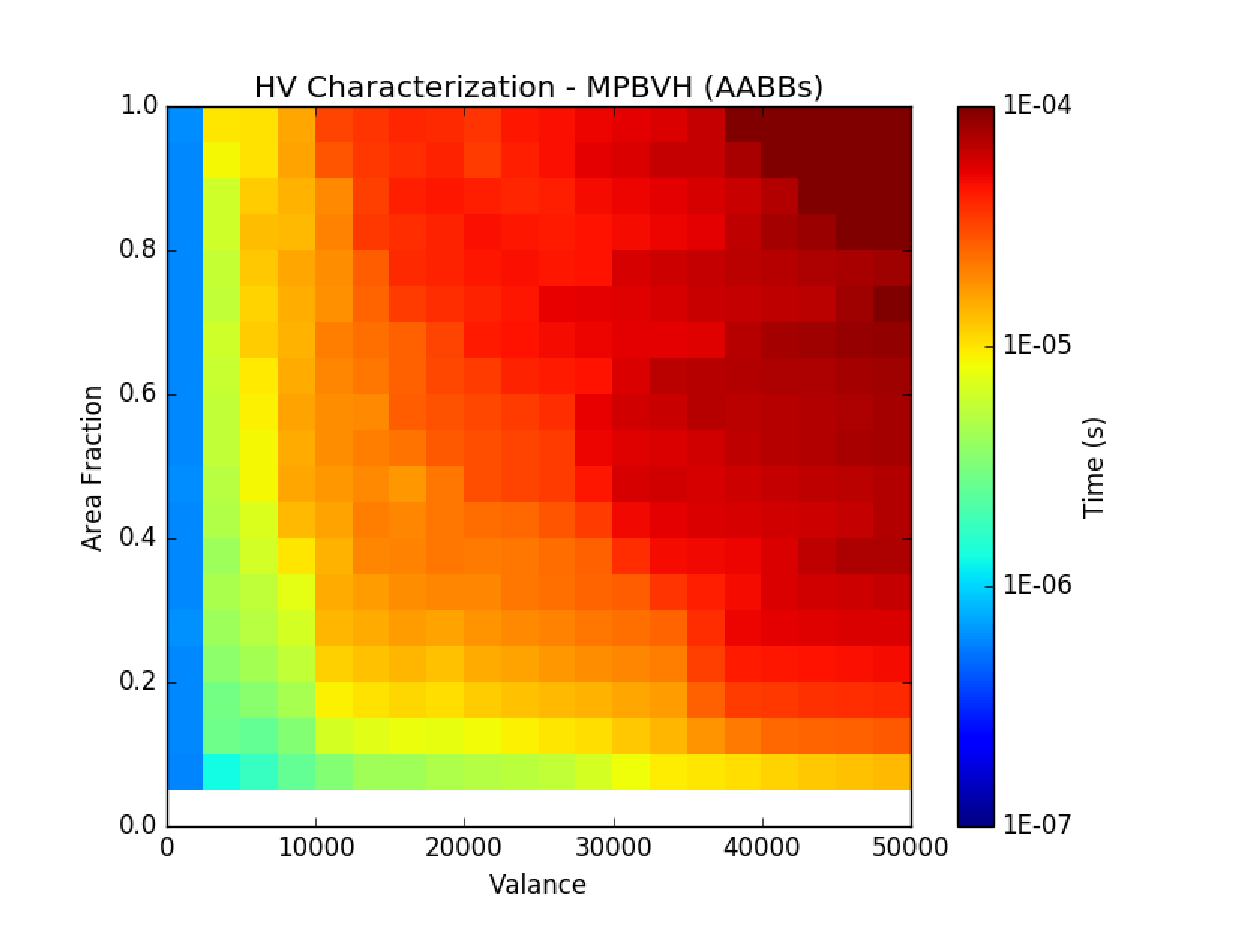
\includegraphics[scale=0.45]{hv_study_SIMD.eps}
  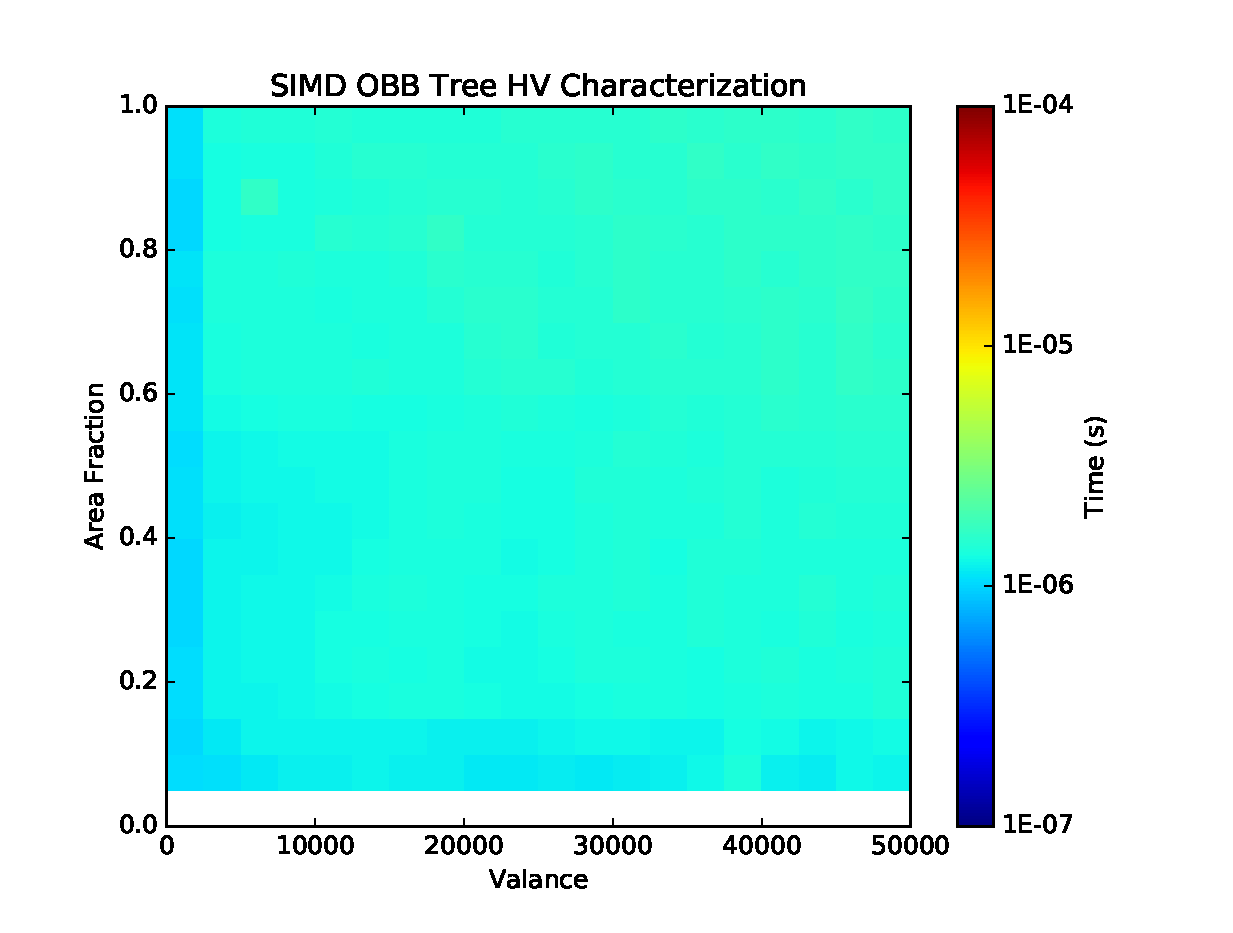
\includegraphics[scale=0.45]{hv_study_SIMD_OBB.eps}
  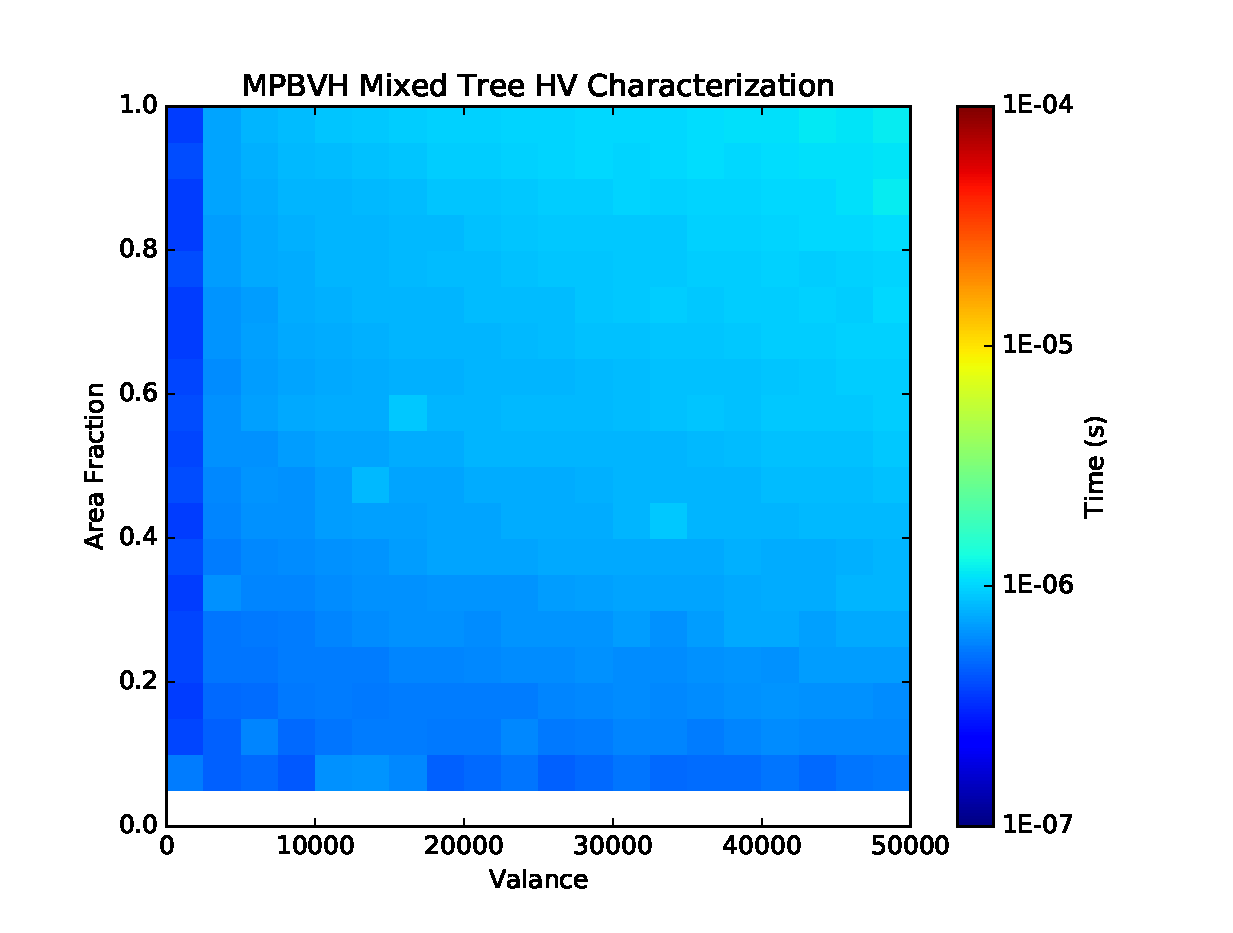
\includegraphics[scale=0.45]{hv_study_mpbvh_mixed.eps}
  \caption[HV characterization studies using EmDAG and MPBVH.]{HV characterization results for all SIMD-enabled ray tracing
    kernels. Top Left: Results of the HV study for EmDAG. Top Right: Results of
    the HV study using the MPBVH with AABBs. Bottom Left: Results using the
    MPBVH with OBBS. Bottom Right: Results for the MPBVH with an adaptive build
    method which applies OBBs in HV regions.}
  \label{fig:simd_hv_studies}
\end{sidewaysfigure}

The information on the frequency of HV leaf visits in Table
\ref{tab:bvhrefine_production_results} was collected on regions of the triangle
mesh identified as high valence during BVH construction as well as
simulation. Leaf nodes in MOAB's OBB Tree determined to be part of high valence
regions with an HV parameter, $\alpha$, equal to 0.5 were tagged. A counter was
incremented each time one of these tagged HV leaf nodes was visited in
simulation, along with counters for the number of total nodes visited and the
total number of leaf nodes visited. The adaptive building method was not applied
to these simulations to avoid biasing the values for leaf node visits. This
lends some insight into the impact of HV regions on DAGMC simulation
performance. It is interesting to note that, in all of these models, HV leafs are
visited rather infrequently, yet they still have a significant impact on the
performance of the simulation. This isn't surprising given the severity of the
ray fire performance degredation seen in Figure \ref{fig:moab_hv_studies}.

\subsection{Embree's Ray Tracing Kernel}\label{sec:emdag_hv_study}

For all of the tests and simulations performed in Chapter \ref{ch:simd_bvh},
EmDAG was much faster than DAGMC. Using the same ray fire test program in EmDAG,
the HV characterization study was performed with somewhat surprising results. 

%% Upon visually inspecting the faceted FNG model, it was
%% seen to contain many HV regions. As an artifact of the variance
%% reduction used in the intended analysis of this model, many planes were inserted
%% in the model in order to break up large cells with highly varying particle
%% intensities. Where these planes intersect the cylindrical volumes of the model,
%% many HV regions result as can be seen in Figure
%% \ref{fng-faceted-models}. As a result it became a curiosity as to whether or
%% not the HV regions were being handled better by EmDAG than they were
%% by DAGMC. In order to test this, the same programs used to do the HV
%% vertex study were built using EmDAG and the parameter study of the relative high
%% valence area and valency was performed. The results in Section \ref{sec:emdag_hv_study}
%% show that EmDAG also struggles with these HV regions. In the worst
%% scenario there is a degradation by two orders of magnitude compared to the best
%% case scenario which is similar to what seen in the unmodified MOAB ray
%% tracer. Additionally, it shows degraded performance in the same way that DAGMC
%% was initially expected to falter - with increasing HV area and
%% valency. This is likely due to the nature of the heuristics used by Embree to
%% construct its acceleration data structures.  Unlike MOAB, however, the BVH
%% building parameters are not as openly available via Embree's interface.There is,
%% however, an option to reduce the size of the HV regions in the mode
%% within the faceting algorithm by defining a length tolerance.

%% \begin{figure}[H]
%%   \small
%%   \begin{center}
%%     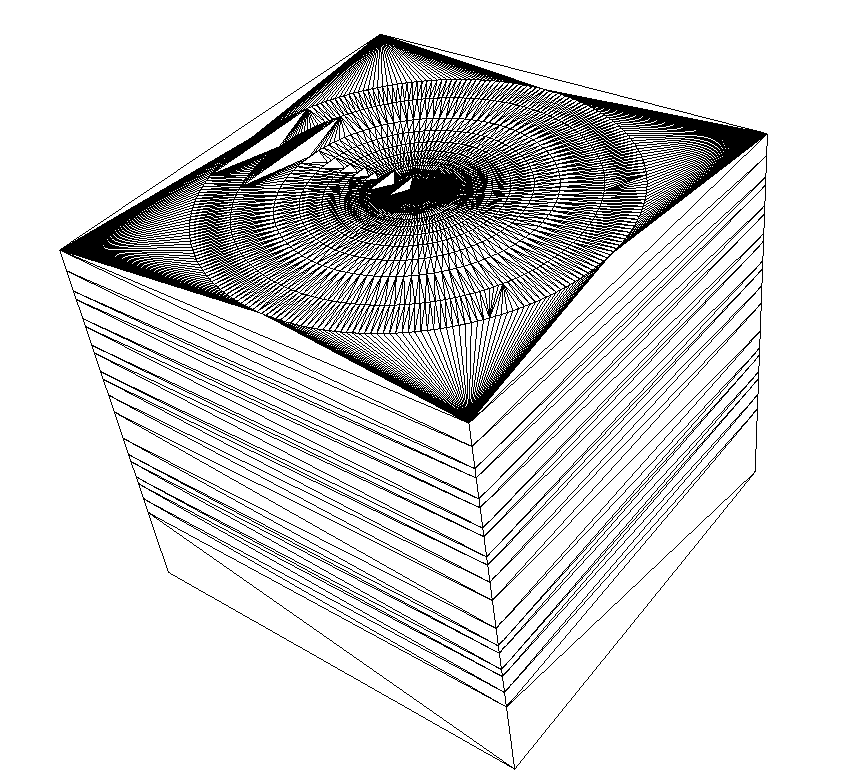
\includegraphics[scale=0.3, trim = 200 0 100 0]{fng_facet_tol.png}
%%     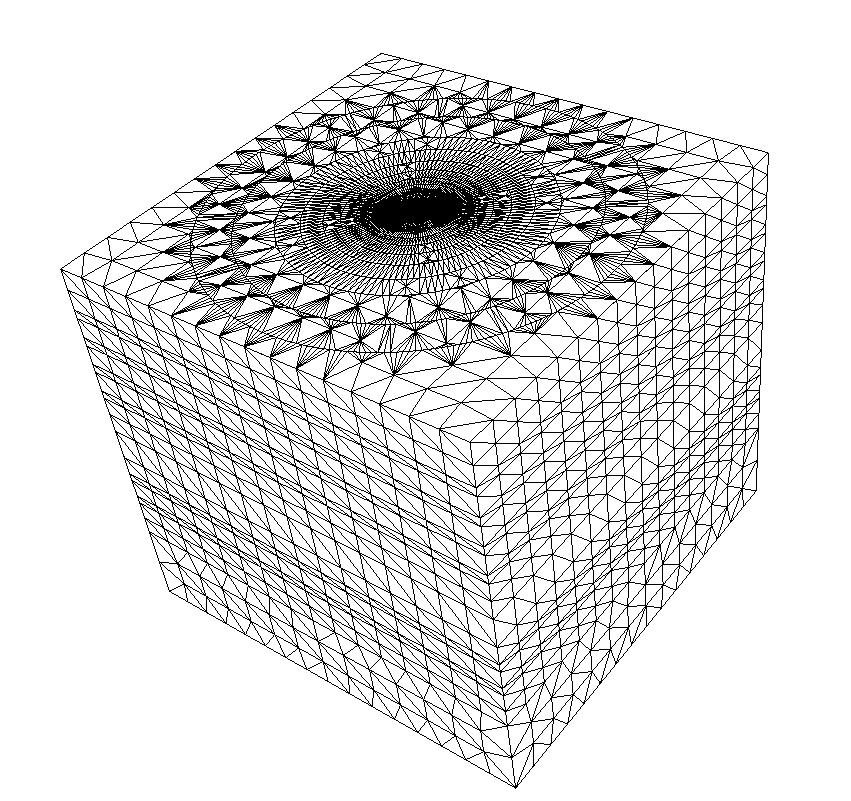
\includegraphics[scale=0.25]{fng_len_tol.png}
%%     \caption{The FNG faceted model without (left) and with (right) the length
%%       tolerance applied.}
%%     \label{fng-faceted-models}
%%   \end{center}
%% \end{figure}

%% The length tolerance is a maximum length for any facet edge returned by the CAD
%% engine's faceting algorithm. Providing this value to the preprocessing tool
%% comes at the cost of many more triangles than when supplying only a faceting
%% tolerance. The difference in facet structure between these models can be seen in
%% Figure \ref{fng-faceted-models}.

%% \begin{table}[H]
%%   \small
%%   \begin{center}
%%         \begin{tabular}{|c|c|c|c|c|}
%%       \hline
%%       \textbf{Implementation} & \textbf{ctme (min)} & \textbf{wall time (min)} & \textbf{ratio} & \textbf{lost} \\
%%       \hline
%%       MCNP5 & 209.92 & 205.99 &  1.00 & 0 \\
%%       \hline
%%       DAG-MCNP5 (lt) & 974.99 & 974.75 & 4.73 & 0  \\
%%       \hline      
%%       EmDAG-MCNP5 (lt) & 257.49 & 257.60  & 1.25 & 247 \\
%%       \hline
%%     \end{tabular} 
%%     \caption{A comparison of transport on the FNG model using a 14.1 MeV
%%       volumetric source over 100M histories for native MCNP, DAG-MCNP, and
%%       EmDAG-MCNP. The DAGMC model was faceted using a length tolerance to
%%       mitigate the effect of HV regions.}
%%     \label{fngemdag}
%%   \end{center}
%% \end{table}

%% By generating a faceted model using the combination of the length and faceting
%% tolerances it was hoped that there would be a marked increase in performance
%% using the EmDAG system and the performance did indeed improve by ~15\%. Due to
%% the increased number of overall triangles on these planar surfaces, there may be
%% competing forces at play. As the length tolerance is reduced, the HV
%% areas will also be reduced, but the overall number of triangles will increase -
%% resulting in inherently deeper BVH and longer traversals. Conversely, as the
%% length tolerance is increased, the number of HV region areas are
%% increase, but the number of redundant triangles is reduced improving the average
%% BVH traversal time enough compensate for a few more rays entering HV
%% regions. This observation leads to the idea that length tolerance of the FNG
%% model could then be optimized. This optimization study, while interesting, will
%% vary model to model and the results will be complex in nature, depending on the
%% underlying geometry and geometry adjacent to those regions, etc. In light of the
%% HV study results indicating that BVH building parameters can be altered
%% to improve performance and accommodate these HV regions, it seems that
%% a better solution is to follow that path over alteration of the mesh globally in
%% the model.

%% This study indicates that the simulation improves when faceting with a length
%% tolerance, but isn't conclusive about the impact of HV regions on
%% EmDAG's ray tracing performance. To better understand this impact, a
%% characterization of EmDAG's reponse for HV regions was conducted.

\subsection{High Valence Characterization}

The same test described in Section \ref{sec:hv_study_MOAB} was performed using
the ray fire test program compile with using EmDAG to fire rays. A different
behavior was expected when using Embree to construct the underlying hierarchies
due to its use of the SAH. Figure \ref{fig:simd_hv_studies} contains the results
of this test run. Using the Embree kernel, the performance degrades in direct
proportion to both valence and the relative area of the HV region. This data
presents the behavior originally expected of MOAB's BVH. Unlike MOAB however,
Embree's use of the surface area heuristic prevents the artificial increase in
probability of visiting triangles in the HV region. Larger triangles adjacent to
this region are more readily separated from the leaf due to the additional cost
they add by increasing a bounding box's surface area and in turn its evaluated
cost. Separation of triangles in the HV region itself is still difficult when
restricted to axis-aligned candidate split planes.

While this data provides evidence that HV regions are problematic for
production-level ray tracing kernels, it is difficult to employ any adaptive
tree construction techniques. Without access to the underlying mesh
representation of the triangle surface, it is difficult to detect HV regions as
implemented in MOAB's OBB tree. This is both a strength and weakness of Embree's
design in that it can build highly efficient data structures using only
primitive point and connectivity data, but it has no infrastructure in place to
interrogate the mesh more deeply. Methods for detecting and adapting to these HV
regions are addressed using the MPBVH, a system with similar characteristics
but with more access to the mesh interface. Due to the similarity in design and
use of AABBs, the MPBVH will act as something of a surrogate for the EMDAG in
terms of its response to HV regions.

\section{Mixed Precision Bounding Volume Hierarchy}\label{sec:simd_hv_study}

\subsection{High Valence Characterization}

The MPBVH kernel created by the author has a similar trend to Embree's kernel
where ray fire times increase proportionally to both the valence and size of the
HV region as seen in Figure \ref{fig:simd_hv_studies}. The author's BVH applies
a modified form of the surface area heuristic as described in Section
\ref{sec:ssah}. Near HV regions this heuristic is able to separate large
triangles from the HV region in the same way as the unmodified surface area
heuristic from Section \ref{sec:heuristics}, but it fails to create a
well-structured tree for triangles that are part of the HV area.

\subsection{Visualization and Diagnosis}

\begin{figure}
  \centering
  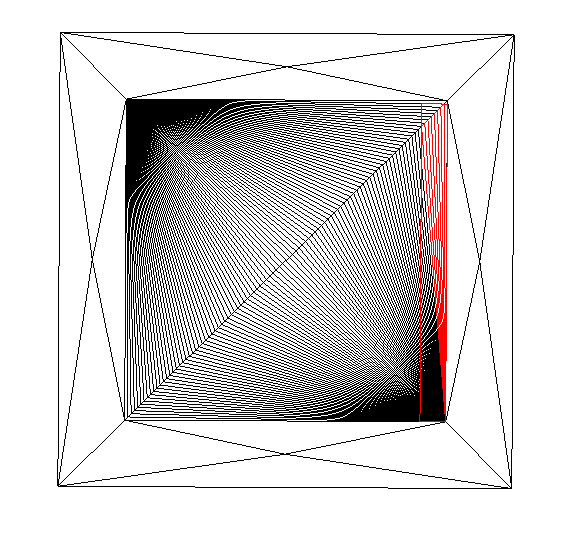
\includegraphics[scale=0.5]{hv_leaf_simd_bvh.png}
  \caption[Axis-aligned bounding box in the high valence region.]{MPBVH
    Axis-Aligned leaf node for the HV test model with area fraction 0.5 and a
    valence of 100.}
  \label{fig:hv_leaf_simd_bvh}
\end{figure}
  
Both Embree and the MOAB SIMD BVH have the shared characteristic of maximum leaf
size of eight primitives due to the way the leaves are encoded. This removes the
possibility that large numbers of triangles in leaf nodes as the cause of
performance degradation, which was the case for MOAB's OBB Tree. For Embree and
the MPBVH, the largest cause of performance degradation is overlapping regions
of the leaf nodes.

Because both of these implementations use AABBs, bounding of high aspect ratio,
off-axis triangles results in bounding boxes with a considerable amount of empty
space in them. An example of such a leaf can be seen in Figure
\ref{fig:hv_overlap_simd_bvh}. In HV regions, this results in the same
space being occupied by a high number of leaf bounding boxes. If a ray is fired
into these overlapping leaves, the end result is a large number of leaf nodes,
and in turn, triangles, visited.

\begin{figure}
  \centering
  \begin{subfigure}{.5\textwidth}
    \centering
    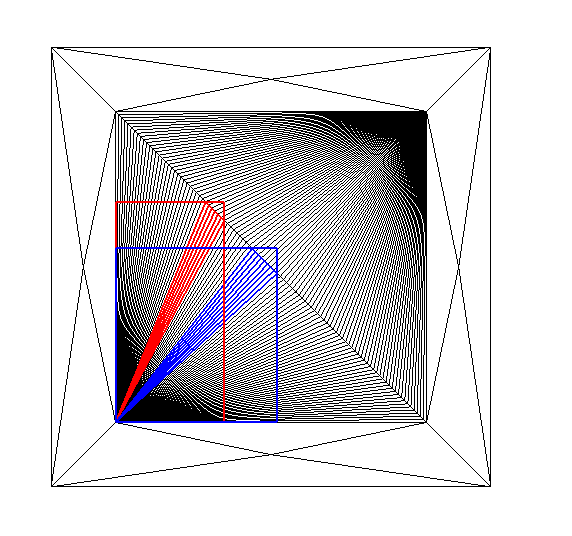
\includegraphics[scale=0.37]{hv_overlap_simd_bvh.png}
  \end{subfigure}%
  \begin{subfigure}{.5\textwidth}
    \centering
    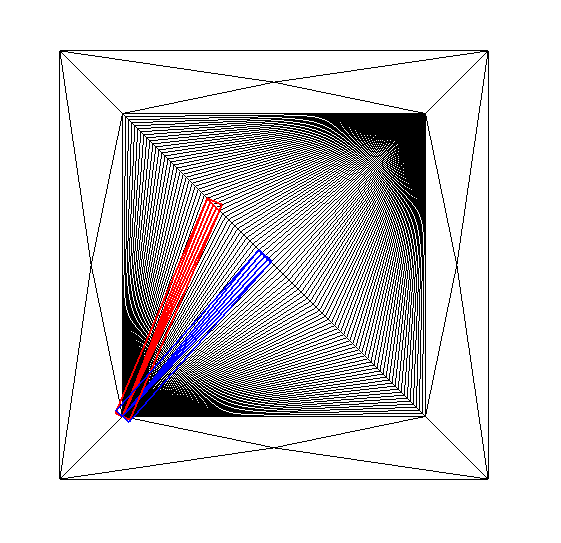
\includegraphics[scale=0.37]{hv_obbs.png}
  \end{subfigure}
  \caption[Bounding boxes of the MPBVH in the high valence
    region.]{Visualization of both axis-aligned and oriented boxes surrounding
    low aspect ratio, off-axis triangles.}
  \label{fig:hv_overlap_simd_bvh}
\end{figure}

To alleviate the effect of the overlapping AABBs in this region, OBBs were
implemented as part of the MPBVH. Figure \ref{fig:simd_hv_studies} shows the
results of the HV characterization study using only OBBs. Because the simplified SAH heuristic is able to separate
large triangles exterior to the HV region into different leaf nodes and the
maximum leaf node size is predetermined, scaling very similar to the MOAB OBB
implementation after HV refinement is applied can be seen, though the overall
speed is somewhat improved due to the single precision implementation.

\subsection{Adaptive BVH Construction}

\subsubsection{OBB Implementation}

The same co-variance method used in MOAB to construct OBBs was applied in the
MPBVH \cite{Weghorst_1984}, but the storage technique used differs in order to
accommodate the SIMD programming involved in the BVH traversal. OBB nodes are
stored as scaled, affine transformations of the global problem space and the
box's lower left corner is stored as a scaled reference point in the oriented
coordinate system. When a ray is intersected with a node it is transformed and
scaled at the same time, but separately, for each of the four OBBs the node
represents. A reciprocal direction is then calculated with respect to the
oriented axes of each box. After this transformation, intersection values and
distances are then returned in the same way they are calculated for a node of
AABBs \cite{Wald_2014}.

As discussed in Chapter \ref{ch:background}, OBB nodes contain additional
information in the form of the affine space transformation and are more
computationally expensive when computing ray transformations. Some of this
computational cost is avoided by incorporating the spatial scaling of the node
into both the affine space and reference point to avoid the additional
computational cost of scaling the parametric values of the ray intersection
later in the calculation.

\subsubsection{OBB Ray Fire Testing}

Tests of the raw ray fire speed using only OBBs were performed using the
MPBVH, which can be seen in Figure
\ref{fig:rf_test_results_obbs}. These tests were conducted primarily as
verification that the exclusive use of OBBs results in a slower ray fire times. 

\begin{figure}[H]
  
  \begin{subfigure}{0.5\textwidth}
    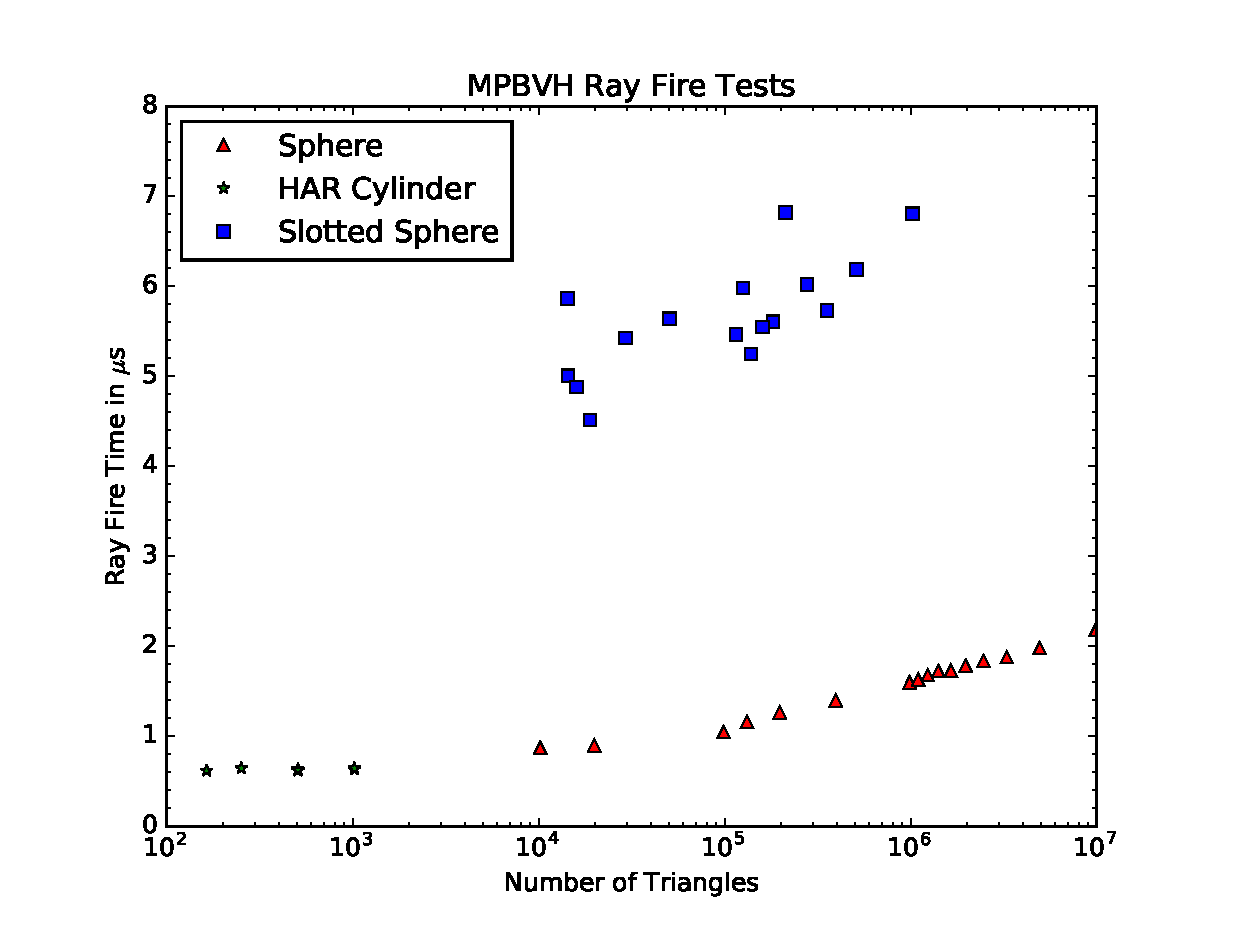
\includegraphics[width=\linewidth]{mpbvh_rf.eps}
  \end{subfigure}%
  \hfill
  \begin{subfigure}{0.5\textwidth}
    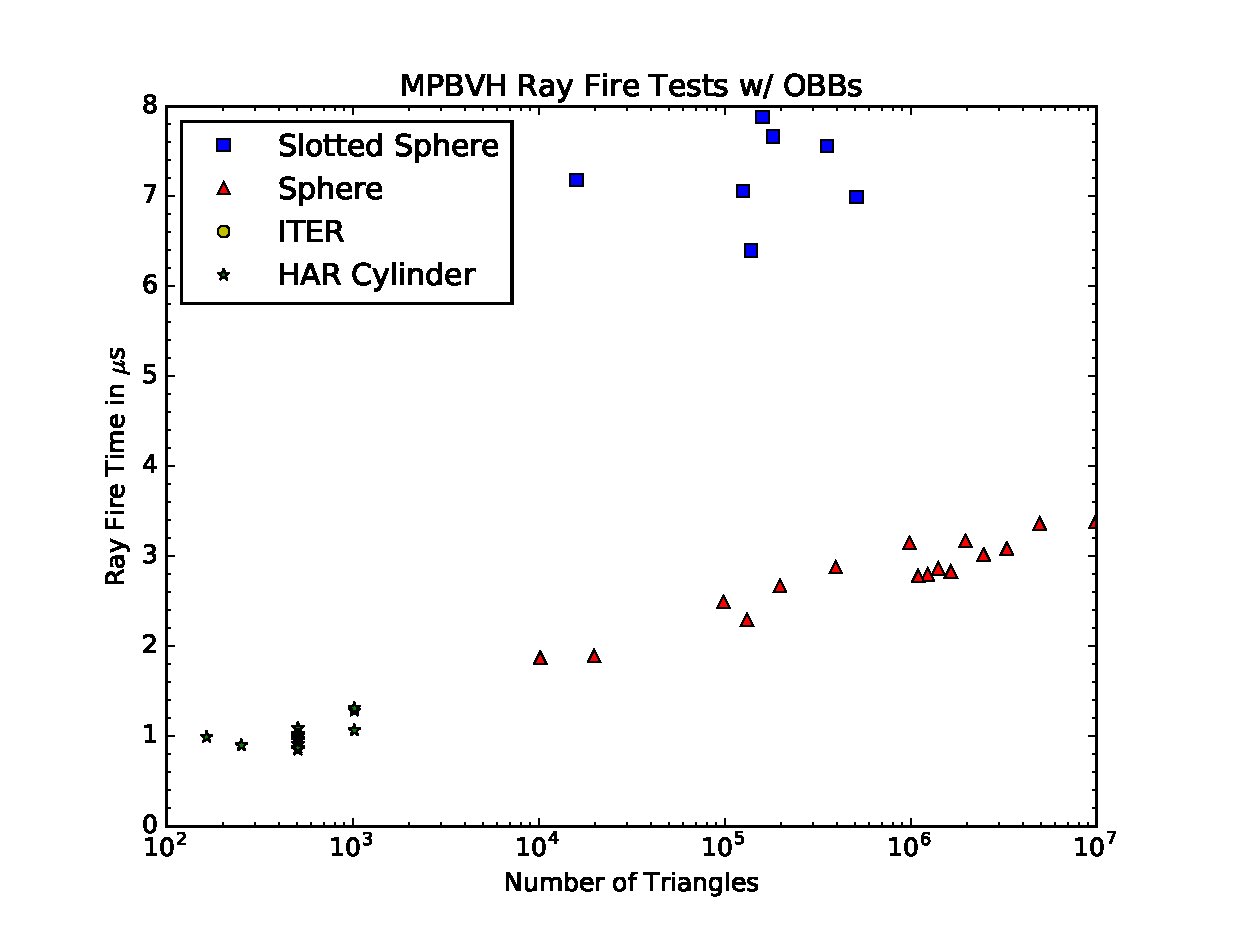
\includegraphics[width=\linewidth]{mpbvh_rf_obb.eps}
  \end{subfigure}
  
  \caption[Ray fire timings for the MPBVH with oriented bounding boxes.]{Ray
    fire tests on three representative DAGMC volumes. Each data point represents
    the average ray fire time for 600k randomly directed rays from the origin of
    each volume. Left: MPBVH with AABBs only. Right: MPBVH with OBBs only.}
  \label{fig:rf_test_results_obbs}
\end{figure}

On average, the ray fire times using OBBs only were about two times slower
than those using only AABBS. The combination of the MPBVH leaf
examination in HV areas with the slower ray fire times of OBBs in the
common case leads to the conclusion that OBBs can be beneficial to ray fire
times, but only if they are used in regions of the model where sibling
AABBs contain large overlaps for these pathological mesh features. 

\subsubsection{A Mixed AABB/OBB BVH}

The solution to HV regions when using the SIMD BVH
kernel proposed by the author is to apply OBBs only in regions determined to be
HV using the same detection method described in Section
\ref{subsubsec:hv_detection}. Large leaf nodes being split into smaller nodes
will apply oriented bounding boxes to contain entities if the set of triangles
is determined to be a HV region using the same method discussed in
Section \ref{subsubsec:hv_detection} for MOAB's OBB tree. The results using the mixed tree with
OBBs applied in HV regions are shown in Figure \ref{fig:simd_hv_studies}. The
mixed tree implementation shows some slight degradation in speed with both area
fraction and valence, but overall timing is significantly better, with the worst
case timing still beating out the best case for the OBB-only characterization
test. This indicates that the AABBs are accelerating intersections higher up in
the tree while the OBBs resolve the HV region with minimal overlap,
resulting in an overall improvement in the run times for these regions.

To support a tree containing both AABBs and OBBs, additional encoding of
interior nodes is required so that the appropriate node intersection methods are
applied during traversal. Axis-Aligned and Oriented nodes are identified using
the two remaining bit configurations available for node definitions by
setting the appropriate bits in the node reference objects. These node masks are
stripped from the node reference's integer value to retrieve the pointer to the
node objects themselves with little added overhead in the traversal process.

\subsubsection{Application to Production Models}

The Mixed MPBVH was applied to the same set of production transport tests as the
AABB MPBVH in Section \ref{subsec:mpbvh_production_transport}. Timing results of
these simulations can be found in Figure \ref{fig:hv_parameter_study_mpbvh}.

\begin{figure}[H]
  \centering
  \includesvg{../images/hv_parameter_study_mpbvh}{width=1.0\textwidth}
  \caption[High valence detection parameter study using the MPBVH.]{Variation in run time for
    different HV detection parameters on a representative set of DAGMC models
    using the MPBVH.}
  \label{fig:hv_parameter_study_mpbvh}
\end{figure}

The application of OBBs in HV regions makes little difference in the simulation
run times of ATR or UWNR, but in the FNG model and ITER model the run times are
reduced by up to ~40\% with little additional build times in the BVH and
minimal increase in the memory footprint by replacing some of the AABBs with
OBBs. This reflects the behavior seen in results of Table
\ref{tab:bvhrefine_production_results} for simulations using MOAB's OBB tree. A
study on the HV leaf visit frequency was not performed here due to a limited
ability to mark HV leaf nodes in the MPBVH system.

%\begin{table}
%  \small
%  \begin{center}
%  \begin{tabular}{lcccccccc}
%    \toprule
%    Model & \thead{Regions \\ Identified} & \multicolumn{3}{c}{HV Area
%      ($cm^{2}$)} & \multicolumn{3}{c}{HV Valence} & \thead{HV Leaves / \\ Leaf
%      Visit \%} \\
%         &      & Max    & Min   & Avg    & Max  & Min & Avg    &      \\
%    \hline
%    FNG  & 514  & 1786.3 & 0.013 & 12.91  & 521  & 14  & 179.9  & 3.83 \\
%    ATR  & 836  & 52.74  & 0.01  & 1.86   & 519  & 14  & 58.735 & 0.07 \\ 
%    UWNR & 499  & 168479 & 0.03  & 2496.3 & 1041 & 31  & 31.63  & 3.87 \\
%    ITER & 3522 & 853827 & 0.02  & 1363.4 & 3082 & 12  & 93.3   & 7.34 \\
%    \bottomrule
%  \end{tabular}
%  \end{center}
%  \caption[High valence region simulation statistics.]{High valence
%    identification and visit statistics for several DAGMC production models. The
%    high valence parameter, $\alpha$, was set to 0.5 for this study.}
%  \label{tab:hv_simulation_stats}
%\end{table}

\section{Summary}

This chapter introduced performance degradation caused by a tessellation feature
seen in engineering models for CAD-based MCRT-t. A test model was then
developed to characterize and study the underlying cause of this degradation for
several ray tracing systems. In MOAB's OBB tree, the main cause was leaf nodes
containing large numbers of triangles. The cause of poor ray tracing performance
in this system was a combination of the tree's design and default splitting
heuristic. A simple HV detection algorithm was presented and applied in a
solution where build settings of the splitting heuristic are adjusted for
portions of the tree bounding HV regions. This method was then verified to
remove performance degradation of ray tracing performance in these regions. A
similar process was then repeated for both EmDAG and MPBVH.

In the MPBVH, and presumably in EmDAG, the exclusive use of AABB nodes results
in large overlaps between child boxes. Many negative triangle intersections
result from these overlaps, a similar effect to containing many
triangles in a single leaf node. The solution proposed and verified by the
author is the use of OBBs only in HV regions by applying the same HV detection
method as was used in the MOAB OBB tree. It is important to note, that this was
only possible in the MPBVH due to it's application alongside MOAB, a fully
formed mesh database. The use of mesh-specific concepts such as element
adjacencies makes this detection method simple and efficient. This work was not
duplicated in Embree due to the difficulty involved in obtaining the same set of
information and application of a mixed BVH for ray tracing on triangle elements.

Finally, a study of the adaptive build method to production models is presented
for understanding of the HV parameter's effect on simulation run times. Little
impact was found for some models while a significant reduction was seen in
others. It was also was found that these run times are significantly reduced
despite the fact that a very small number of rays are intersected with triangles
in HV regions as shown in Table \ref{tab:bvhrefine_production_results}.

\section{Future Work}

For the models studied in this chapter, any HV detection parameter below 1.0 was
shown to be effective in reducing simulation run times. This parameter could be
studied and optimized using a broad range of test cases to determine the best
value for use in the general case.

Alternative methods to reducing the HV performance pathology could be explored
as well. Here, BVH data structures were modified to better suit the HV mesh
feature. Conversely, the HV regions could also be modified to better suit the
BVH. A re-meshing of the HV region to contain a more uniform tessellation would
allow a BVH of AABBs to maintain traversal performance without modification to
the BVH build, though this would presumably come at the cost of more triangles
in the model. Re-meshing of HV regions was not explored in this work due to the
concerns for the additional memory cost outlined in Section \ref{sec:mc_mem}.
